\documentclass[lof,los,12pt,progress]{puseniorthesis}
% options to class:
% lof - generate list of figures
% lot - generate list of tables
% los - generate list of symbols
% Xpt - font size
% filecopy - note that this is 'File Copy' on title page
% advisercopy - note that this is 'Adviser Copy' on title page
% readercopy - note that this is 'Reader Copy' on title page
% progress - title page has 'Progress Report' instead of 'Final Report'

\usepackage{xcolor}
\usepackage{graphicx} % needed for \includegraphics
\usepackage{amsmath}
\usepackage{float}

% required inputs:
\author{Katherine Denner}
\classyear{`19}
\adviser{Daniel Steingart}
\reader{My Reader}
\title{Identification of lithium deposition and characterization of state of charge and health in extreme fast charge cells using ultrasonic methods}
\dept{Mechanical and Aerospace Engineering}
\submitdate{Sometime in the future}
\course{MAE442}
\abstract{%%
%% MOTIVATION
%%
High performance batteries such as those critical to electrical vehicle adoption require constant, accurate estimation of many cells' state of charge and state of health, and deft management of the battery based on that information is critical both to vehicle performance and safety. 
Inadequacies in the state of the art are holding back more widespread electric vehicle adoption. 

This thesis builds on prior work in developing new, ultrasonic methods for measuring battery state of charge and state of health in operando, and for the first time demonstrates the technology's ability to measure ambient temperature, a key metric for both performance and safety in electric vehicles.
Prior work in this area targeted standard consumer battery formats such as AA. 
The fast-charge batteries favored by high-performance applications such as electric vehicles present additional challenges due to their more rapidly-shifting properties and more compact form factors, yet also present greater opportunity because so much more can be gained by improving their performance. 
The work herein focuses on extreme fast-charge cells, but its results can be generalized to other cells which are easier to work with.

Described within is the design of an experimental apparatus was designed tp allow for electrically manipulating the lithium-ion cell's state of charge and state of health while regulating its ambient temperature and pressure; the experimental procedures used to explore the validity of these acoustic time of flight techniques to lithium-ion fast-charge cells; and the data analysis used to synthesize and interpret acoustical, electrochemical, and thermal data.

Ultimately, this thesis demonstrates the capability of acoustic time of flight analysis to observe changes in the state of charge and state of health in a fast-charge lithium-ion cell, and for the first time, to observe changes in the cell's ambient temperature.}

%\extranotes{These are a few lines of optional notes} 
\dedication{To myself.}
\acknowledgements{Thank you very much.}

\numberwithin{equation}{section}

\begin{document}

\chapter{Introduction}

\section{Motivation}
Increasing demand for electric vehicles is pushing the need for extreme fast charge capabilities in lithium battery chemistries, and a critical limiting factor in charging rates is lithium deposition \cite{XFC}. Charging a lithium battery too quickly causes lithium deposition, which reduces cell capacity and in severe cases, creates safety hazards \cite{XFC}. Currently there is no practical in operando method of detecting lithium deposition. Without real-time lithium deposition monitoring, safety and financial considerations require batteries with lithium-based cells to use controllers programmed to charge and discharge conservatively. Being able to monitor lithium plating would allow battery management systems for lithium cells to more accurately control charging rates, and potentially even employ charge and discharge protocols that unplate lithium.

The objective of this thesis is to use ultrasonic methods to demonstrate the feasibility of detecting the deposition of lithium and determining changes in the state of charge and state of health of single layer, high-rate lithium ion cells.

%% broad introduction
% when choosing what to include, assume the reader will only skip it
%   include any critical background in a subsection of the relevant chapter
\chapter{Background}

\section{Lithium Ion Fast Charge Cells}

\subsection{Lithium Ion Battery Chemistry}
Increasing demands on the energy density and form factor of rechargeable batteries created a massive and growing market for lithium ion battery cells \cite{LBST}. 
Their superior gravimetric and volumetric energy densities are due to the high cell voltages (~4V), which are made possible by the non-aqueous electrolytes of lithium cells \cite{LBST}. Batteries work by passing ions back and forth between two electrodes - separated, charged materials. In its fully charged state, a battery cells charge has collected on its negatively-charged electrode (the anode). 
The ions are keen to flow to a lower energy state, and flow readily to the positively charged electrode (the cathode), shedding their electrons to the circuit in the process and powering the connected device. 
As more of the ions jump to the cathode, the energy imbalance between the two plates shrinks, until charged particles are no longer easily motivated to move from the anode to the cathode. 
In a rechargeable battery, this process is reversible, and if electrons are fed back to the cathode by reversing the circuit, ions will flow back to the anode \cite{ LBST}. In a lithium ion battery, these ions are Li$^+$. \todo{get cell chem}.

The voltage of a battery is simply its potential energy per charge, and the open-circuit voltage $V_{oc}$ of a lithium-ion cell is a function of
$$ V_{oc} = \frac{\mu _{Li(c)} - \mu _{Li(a)}}{F} $$
where $\mu_{Li(c)}$ is the lithium chemical potential of the cathode, $\mu_{Li(a)}$ is the lithium potential of the anode, and $F$ is Faraday's constant (the charge in Coulombs of one mole of electrons) \cite{LBST}.
Good charge and discharge performance requires that the "lithium insertion/extraction process should be reversible with no or minimal changes in the host structure over the entire range $x$ of lithium insertion in order to provide a good cycle life for the cell" \cite{LBST}.

\subsection{Lithium Plating}

\subsection{Charging Protocols}

stage 0: preconditioning

If the cell was deeply discharged, it should first be charged at a very low current, so that minimal heat is generated before the cell is in such a state that it can deal with that heat \cite{DIGIKEY}.

stage 1: constant-current 

Drive the cell at a constant current to get its voltage to 4.2V. The higher the current, the faster this charging stage happens, but also the more damage delivered to the cell \cite{TI}. Charging rates are often limited to 1C, but fast charging can allow for higher rates \cite{TI}.

stage 2: constant-voltage 

Charge with constant-voltage until the current steps down to ~0.1 Amps, at which point charging is complete \cite{DIGIKEY}. Constant-voltage charging prevents overcharge \cite{DIGIKEY}. The decreasing current required to maintain 4.2V is what creates the exponential decay shape of the current vs time plots during charging \cite{TI}.

\subsection{Charging Rates}
To normalize across battery capacities, charge or discharge current is often expressed as a C-rate \cite{SPECS}. A C-rate expresses the rate a battery at which a battery is discharged in terms of its maximum capacity; a 1C rate will fully discharge a battery in 1 hour, a C/2 rate will do so in 2 hours, and a 2C rate will discharge a battery in 1/2 hour \cite{SPECS}. Since the cells being investigated in this work have a roughly x Amp-hours \todo{number} capacity, a 1C rate uses \todo{number} Amps for charging, whereas a 10C rate uses \todo{number} Amps.

\section{Acoustic Time of Flight (ToF) Analysis}
Recent work has shown that Acoustic Time of Flight (ToF) Analysis can show the state of charge and state of health of battery cells.

Acoustic ToF analysis probes a unit with continuous acoustic waves, and makes conclusions based on how long it takes for waves to travel to the receiver (either the waves which travel through the test unit to a receiver, or the waves which reflect off of the material and back to the transmitter). How long it takes for a wave to travel from one point to another depends on the ubiquitous relation 
$$\text{distance} = \text{ rate} \times \text{ time} \rightarrow \text{ time} = \frac{\text{distance}}{\text{rate}}$$

Nondestructive ultrasonic analysis measures the time of flight (how long it takes the wave to travel either back to the transmitter, or to a receiver), and the amplitude of the received signal. These quantities can be used to estimate the thickness of the material, $T$:
$$ T = \frac{ct}{2}$$

where $c$ is the material sound velocity, an $t$ is the duration of the flight \cite{OLYMPUS}. 
Thus, if $c$ can be assumed constant, $T$ can be measured using only $t$.
Ensuring $c$ can be assumed sufficiently constant was an important consideration in apparatus design, to be discussed later.

High frequency waves are used because BLANK however BLANK

\subsection{Prior Work}

Hsieh et al \todo{cite?} performed electrochemical-acoustic time-of-flight (EAToF) experiments on batteries of various chemistries and form factors, demonstrating "strong correlation between SOC and the density distribution within a cell, as determined by acoustic measurements" \cite{TOF-STATE}. They go on to conclude that "changes in the ToF echo profiles and acoustic signal amplitudes as a function of cycle number appear to be key indicators of central phenomena occurring within the battery, including changes in intraparticle and interparticle stress and strain, as well as the formation and removal of critical surface layers", suggesting but not demonstrating that electrochemical-acoustic ToF analysis can determine a battery cell's state of health.

That assertion was demonstrated in the subsequent paper by Bhadra et al \todo{cite?} \cite{ANODE-CHAR}, which demonstrated the capacity of electrochemical acoustic time-of-flight analysis to "examine the dynamic properties of cells during discharge" "by tracking the saturation of the central echo and secondary echos, the total shift in the ToF peak position over discharge, and total transmitted signal amplitude".

This work was built on by Davies et al \todo{cite?} \cite{SOC-SOH-EST}, who explored the accuracy of the EAToF method while cycling lithium-ion pouch cells over hundreds of cycles, focusing on "two key metrics: time of flight shift and total signal amplitude, which are the used with voltage data in a supervised machine learning technique to build a model for the state of charge (SOC) prediction". 
In addition to showing their model was about $99\%$ accurate for two different cell chemistries, they showed that the model can be extended to predict state of health with similar accuracy by adding to the model the full ultrasonic waveforms at top of charge.

\todo{Other factors which affect $c$}
What some noise contributions are % \input is a lower-level \include that is typically slower but allows nesting

%input{literature}

%\input{subject} % include pulls form precompiled .aux and is faster than \input, but won't work with labels from other sections; use it when able

%\include{apparatus design}

%\include{electronics}

%\include{firmware}

%\include{experimentation}

%\include{analysis}

%\chapter{Results}

The data clearly show first a relationship between cell state of charge the acoustic TOF through the cell, then between induced lithium plating and changes in acoustic time of flight data, and finally between changes in ambient temperature and change in acoustic TOF through the cell. 

Recall that the three sources of change in acoustic time of flight through a cell are change in state of charge, change in state of health, and change in ambient conditions. 
By systematically adding and understanding changes in each category to the experimental conditions, shifts in acoustic ToF through the cell can be observed, analyzed, and then attributed to each source of change.

When the ambient conditions were steady, the relationship between SoC and ToF was very clear \todo{plot}. Ambient temperature variation clearly has a significant effect on the acoustic TOF shifts. \todo{fig} shows a comparison between the measured TOF data and "idealized" TOF from a gentle, non-plating routine, constructed by assuming the data ought not change between cycles and copying the first waveform repeatedly as a result. In the absence of plating and at the same state of charge, the relationship between change in ToF shift and change in ambient temperature is consistent enough that much of the influence of temperature can be scrubbed out using simple regressions.

\section{Time of Flight Shift Due to Change in State of Charge}
The data clearly demonstrate a strong and consistent relationship between acoustic ToF through the cell and the cell's state of charge while ambient conditions and cell state of health are held steady.

The shift in ToF was determined using a colleague's cross-correlation analysis of each received waveform to a reference waveform. The reference waveform was chosen from one of earliest waveforms in the experiment, but not too early, in order to allow for start-up effects to dissipate.
During the C/2.5 charge and discharge cycling, which does not appreciably plate the cell and therefore can be assumed to not change the state of health of the cell, the ToF data follows a very regular pattern. 
The ToF shift peaks at roughly the same value, and at the same point in the cycling protocol: when the routine finishes charging. 
Conversely, the ToF shift experiences a minimum of fairly consistent value at the end of each discharge period.

\todo{fig}

\section{Time of Flight Shift Due to Change in State of Health}
The data in the same test goes on to demonstrate acoustic TOF analysis's capability to observe plating, and therefore change in a cell's state of health. This is shown during the 5C and especially 10C routines in the experiment. 
While the TOF data maintains a consistent form for each of those protocols, the "neutral axis" to which it returns between cycles increases each time. 
Since the ambient conditions were steady and there was no variation in the cycling protocols, these changes in the TOF shift show lingering changes in the state of health of the cell. 
This is corroborated in each of the experiments. 
SEM (scanning electron microscope) and XPS (X-Ray Photoelectron Spectroscopy) analysis confirm plating on the electrodes of the cells, but such techniques do not provide information on when the plating occurred. \todo{moar}

To confirm plating had indeed occurred, a cell was dissected and used for optical, SEM, and XPS analysis.

\begin{figure}[t]\label{fig:optical}
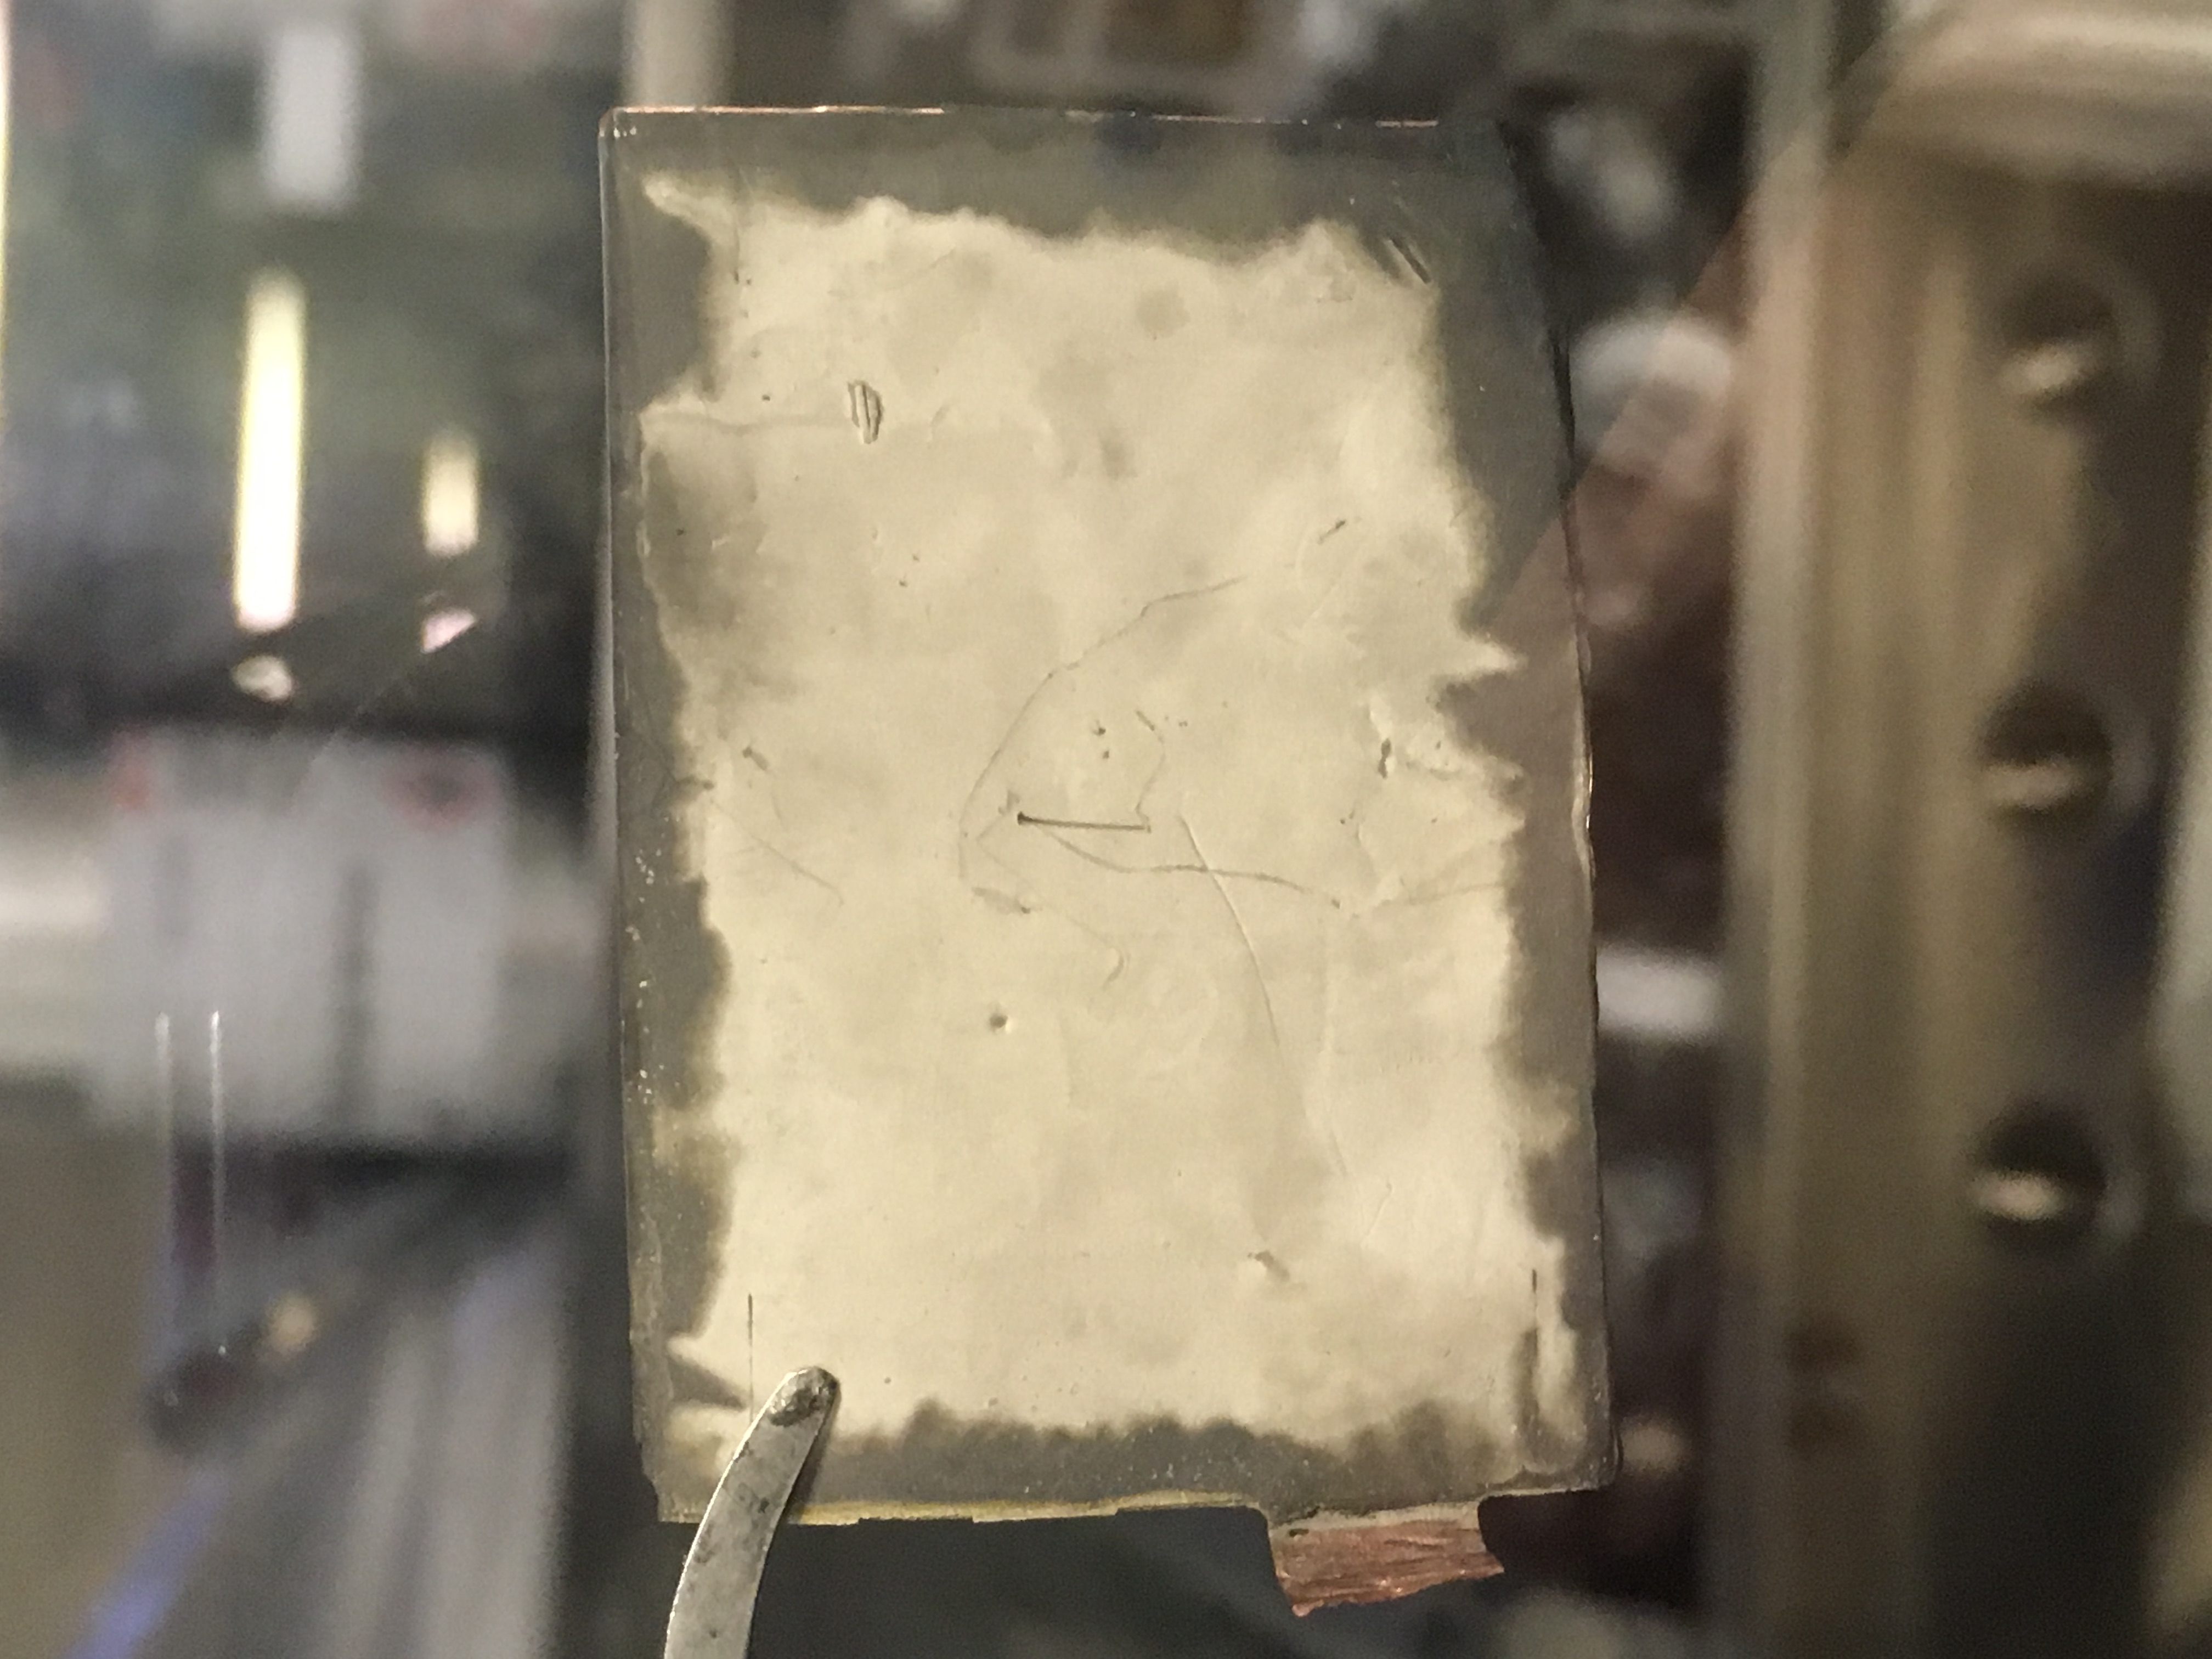
\includegraphics[width=0.6\textwidth]{Thesis/optical.JPG}
\centering
\caption{A cell cut open after electrochemical cycling. The light region is lithiated.}
\end{figure}

Optical analysis provided quick confirmation that the cell had plated; since the cell had not been used before the experimental protocol described above, it can be safely assumed the plating occurred then. SEM and XPS analyses provide more sophisticated information about the plating. 

\section{Time of Flight Shift Due to Change in Ambient Conditions}
In the first experiment which demonstrated the technique, ambient temperature was held quite steady, and had no material impact on acoustic TOF through the cell. 
However, subsequent experiments were unable to maintain such optimal conditions.
During routines using gentle C/2.5 cycling, thus maintaining state of health, the influence of ambient temperature changes on acoustic TOF can be isolated from the influence of state of charge changes with reasonable success. 
Polynomial fits and linear regressions correlate change in ambient temperature with change in ToF shift. 

The thermocouples and transducers have different sampling rates and schedules, so a couple approaches created paired change in ToF shift and change in temperature data; these are plotted against each other in \todo{ref}. 
In one version of the analysis, change in temperature data was averaged across a cycle and regressed against change in TOF shift data. 
More accurate results resulted from interpolating the temperature data using linear or polynomial fits, depending on the shape of the temperature data.

The analysis shows a reasonable estimate at how the ToF would shift without the influence of the ambient temperature shifts, potentially broadening the application of the technique in monitoring cells.
\begin{figure}[t]\label{fig:0417tofshiftadj}
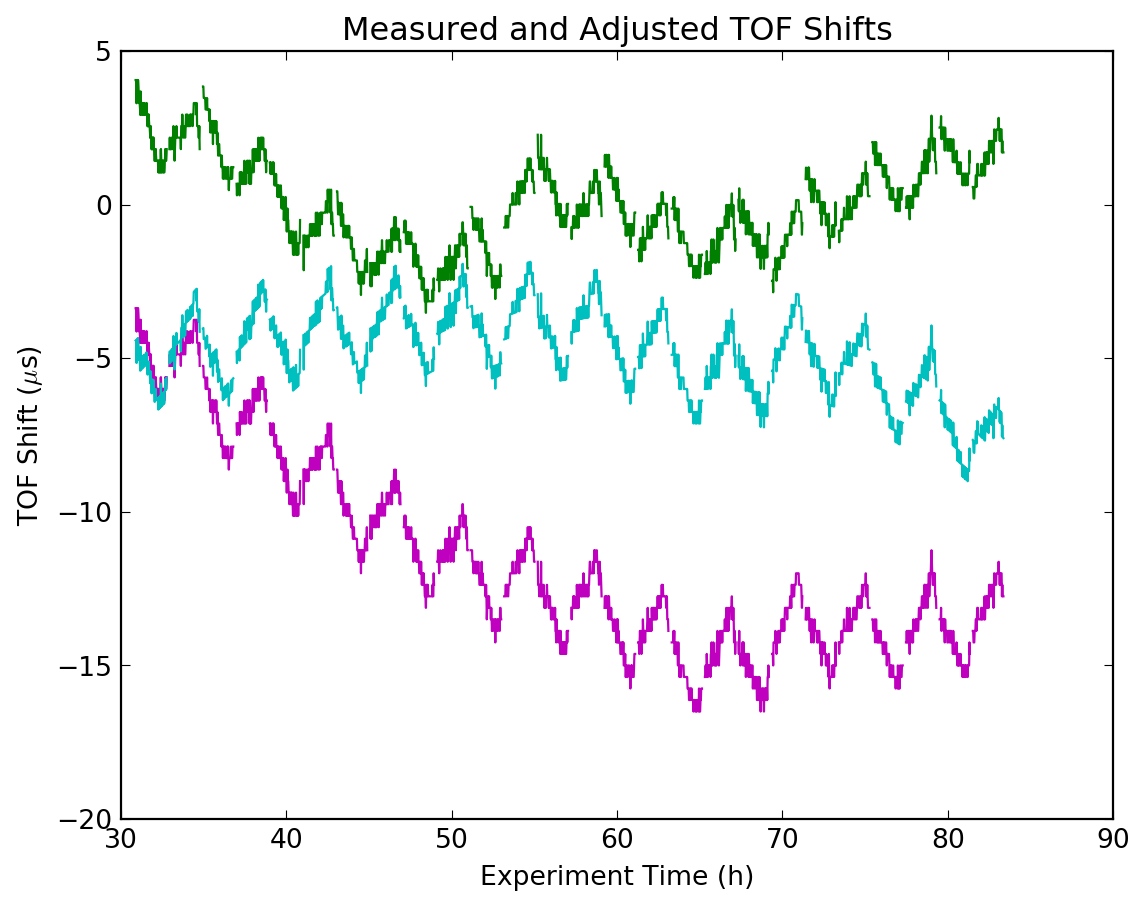
\includegraphics[width=0.75\textwidth]{Thesis/0417tofshiftadj.png}
\centering
\caption{ToF Shift across the experiment. This plot compares the unaltered ToF shift, the ToF shift adjusted using a change in ToF - change in temperature regression using interpolated temperatures, and the ToF shift adjusted using a regression of maximum change in ToF shifts and averaged temperatures.}
\end{figure}

One check is to compare them to an idealized prediction of how the TOF should actually shift during the experiment. 
Since each cycle at a particular charge rate has a consistent duration and consistent effect on the cell's state of charge, it is easy to compare ToF shift data between cycles. 
At any particular point in the cycle's duration, the ToF shift in each cycle should match. Charge and discharge cycle ToF data, when overlaid (see \hyperref[fig:0417overlays]{\cref{fig:0417overlays}}), show how consistent or inconsistent the ToF shifts are across the experiment.
Ideally there would be perfect overlap in the data from each cycle within a protocol within an experiment, but before the ambient temperature shift's influence was removed, this was clearly not the case. 
The overlap is still imperfect after the TOF shift data was adjusted based on the regressions, but it is much better.

\begin{figure}[t]\label{fig:0417overlays}
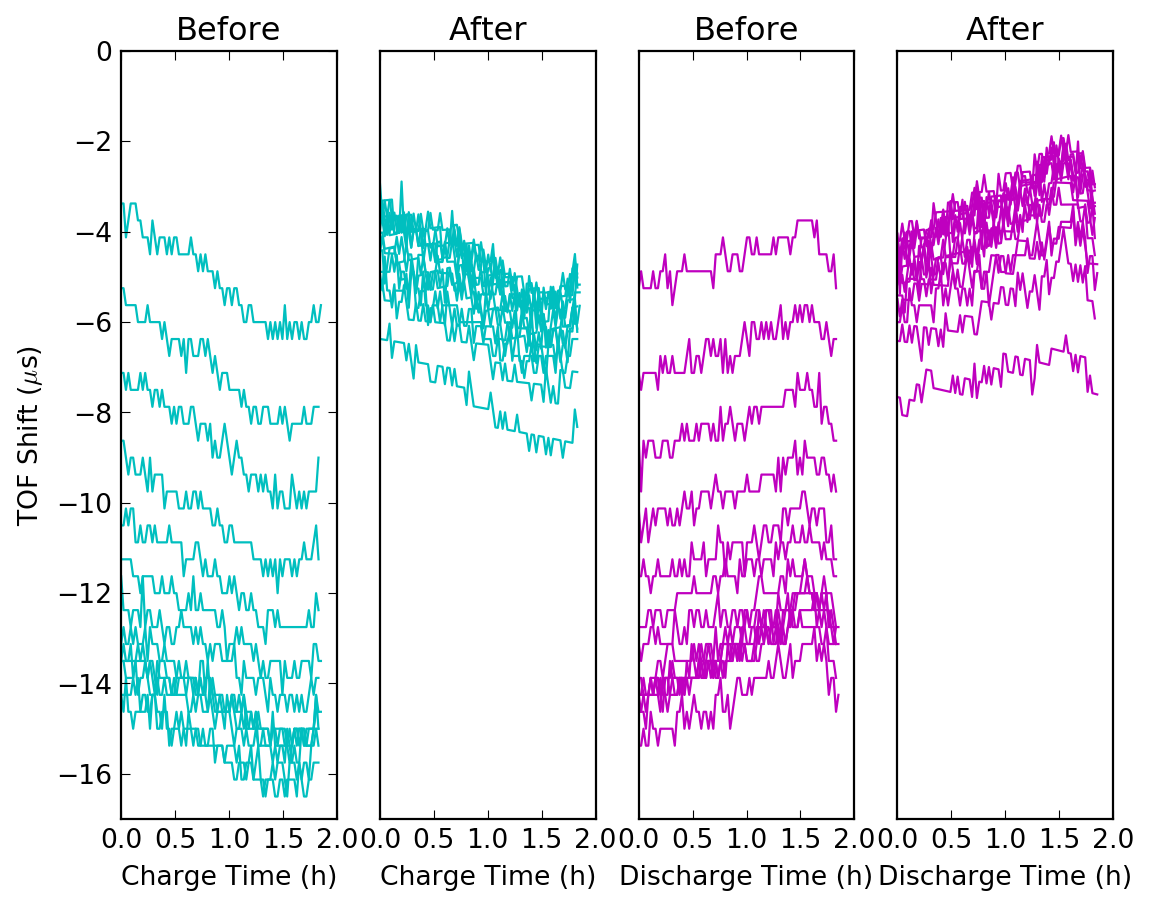
\includegraphics[width=0.95\textwidth]{Thesis/0417overlays.png}
\centering
\caption{Overlays of the raw and adjusted ToF shifts across each charge cycle (far and center left) and discharge cycle (center and far right). The adjusted data used a regression to remove the influence of ambient temperature fluctuations.}
\end{figure}


%\input{discussion}

\bibliography{biblio}
\bibliographystyle{plain}
\nocite{*}

%\appendix

%\chapter{An organ you don't need!}

But would sure like to have!

\end{document}